\icode{N17Q-MD-MU-L2-261111-001}
\nceeID[unkown]{2017海南}{unkown}
（多选）
如图，水平地面上有三个靠在一起的物块 \(P\)、\(Q\) 和 \(R\)，质量分别为 \(m\)、\(2m\) 和 \(3m\)，物块与地面间的动摩擦因数都为 \(\mu\)。用大小为 \(F\) 的水平外力推动物块 \(P\)，记 \(R\) 和 \(Q\) 之间相互作用力与 \(Q\) 与 \(P\) 之间相互作用力大小之比为 \(k\)。下列判断正确的是\paren[]

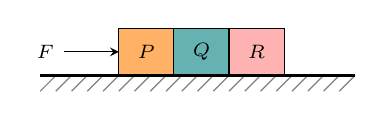
\begin{tikzpicture}[>=stealth,font=\scriptsize]
	\draw[fill=orange!60] (0,0) rectangle(.7,.6)node[midway]{\(P\)};
    \draw[fill=teal!60] (.7,0) rectangle(1.4,.6)node[midway]{\(Q\)};
    \draw[fill=red!30] (1.4,0) rectangle(2.1,.6)node[midway]{\(R\)};
	\draw[->] (-.7,.3)node[left]{\(F\)}--(0,.3);
	\foreach \x in {-1,-.8,...,2.8}
		\draw[gray] (\x,-.2)--++(.2,.2);
	\draw[thick] (-1,0)--(3,0);
\end{tikzpicture}
\begin{choices}
	\item 若\(\mu \neq 0\)，则\(k = \dfrac{5}{6}\)
	\item 若\(\mu \neq 0\)，则\(k = \dfrac{3}{5}\)
	\item 若\(\mu = 0\)，则\(k = \dfrac{1}{2}\)
	\item 若\(\mu = 0\)，则\(k = \dfrac{3}{5}\)
\end{choices}
\begin{answer}
	BD\qquad 提示：
\end{answer}